\subsection{Componentes complementarios}

Dos elementos del circuito de control que valen la pena destacar son:

\begin{itemize}
    \item Relé de 5V: Básicamente sirve como interruptor. Por un lado, se activa utilizando una señal de bajo voltaje, como por ejemplo una tensión continua de $5\,V$. Al activarse el relé, una bobina interna se encarga de abrir o cerrar el interruptor \cite{miguel_diaz}.
    
    \item Regulador de luz: Un regulador de intensidad puede conectarse a un Arduino para controlar la tensión de CA que recibe un dispositivo. El lado de bajo voltaje y el lado de alto voltaje están completamente aislados \cite{regulador_amazon}, lo cual asegura la protección del circuito de control y el microcontrolador.
\end{itemize}

Adicionalmente se presenta a continuación una tabla con todos los componentes electrónicos utilizados y el costo del proyecto:
\begin{figure}[h]
  \centering
  \begin{tabular}[b]{c}
    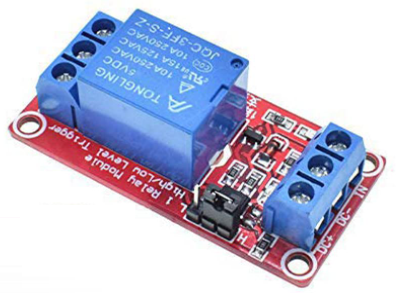
\includegraphics[width=0.35\linewidth]{images/rele.png} \\
    a) Relé de 5V, 1 canal de gatillo de nivel \\ alto o bajo opto aislado \cite{rele_amazon}
  \end{tabular} \qquad
  \begin{tabular}[b]{c}
    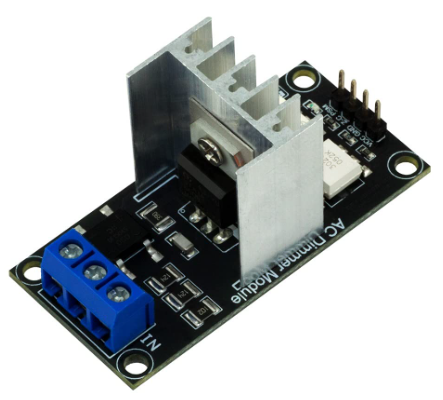
\includegraphics[width=0.33\linewidth]{images/regulador.png} \\
    b) Regulador de luz Arduino de 1 canal \cite{regulador_amazon}
  \end{tabular}
  \caption{Elementos principales del circuito de control}
\end{figure}

\begin{table}[H]
\centering
\begin{tabular}{|cc|c|}
\hline
\multicolumn{1}{|c|}{\textbf{Componente}} & \textbf{Cantidad} & \textbf{Precio (USD)} \\ \hline

\multicolumn{1}{|c|}{Relé}        & 1                 & 1.37                      \\ \hline
\multicolumn{1}{|c|}{Regulador de luz}        & 1                 & 2.93                      \\ \hline
\multicolumn{1}{|c|}{Pantalla LCD}        & 1                 & 5                      \\ \hline
\multicolumn{1}{|c|}{Arduino UNO}        & 1                 & 28.5           \\ \hline

\multicolumn{2}{|c|}{\textbf{Total}}                          & \textbf{37.8}    \\ \hline
\end{tabular}
\label{componentes}
\caption{Lista de cantidad y precios de los componentes (Autoría propia).}
\end{table}

